\section{Theorie}\label{sec:theorie}
Nachdem zunächst auf die verschiedenen Wechselwirkungen von elektromagnetischer Strahlung mit Materie eingegangen wird, folgt mit diesem Wissen eine Einführung in die Funktionsweise des verwendeten Germaniumdetektors.
\subsection{Wechselwirkungsprozesse von Photonen mit Materie}
Im Wesentlichen spielen drei Effekte eine wesentliche Rolle bei dem Einfall von im Versuch erzeugten Gammaquanten in Materie, wie in \autoref{fig:extinkt} dargestellt ist.
Allgemein kann die Intensität $I$ von Strahlung innerhalb eines Materials abhängig von der Eindringtiefe $x$ mithilfe der Funktion
\begin{align}
  I(x) = I_0\cdot\exp{(-\mu x)}
\end{align}
modelliert werden, wobei $\mu$ Extinktionskoeffizient oder Absorptionskoeffizient genannt wird. Dieser von verschiedenen Materialeigenschaften sowie Strahlungsenergie abhängige Paramater beschreibt, wie stark ein Material die respektive Strahlung abschwächt.
Im Anschließenden wird der zustandekommende Graph erklärt.
\begin{figure}[H]
  \centering
  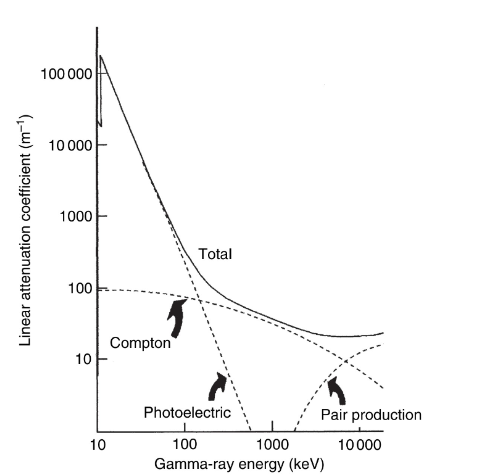
\includegraphics[scale=0.65]{Ressourcen/extinkt.png}
  \caption{Schematischer Verlauf des Extinktionskoeffizienten in Abhängigkeit der Photonenenergie\cite{gilmore}.}
  \label{fig:extinkt}
\end{figure}
\subsubsection{Photoelektrischer Effekt}
Der Photoeffekt beschreibt den Prozess, bei dem ein Gammaquant seine gesamte Energie an ein Hüllelektron eines Atoms abgibt, es herauslöst und das Atom somit ionisiert. Damit es zu diesem Verhalten kommen kann, müssen die Photonen bestimmte Energien, welche mit den Bindungsenergien der Elektronen im Atom übereinstimmen, besitzen.
Der Wirkungsquerschnitt $\sigma$, ein Maß für die Wahrscheinlichkeit eines Wechselwirkungsprozesses, sinkt für den Photoelektrischen Effekt mit steigender Energie, was sich in \autoref{fig:extinkt} in einer Abnahme des Extinktionskoeffizienten $\mu$ widerspiegelt.
Konkret ergibt sich als quantitative Abhängigkeit 
\begin{align}
  \sigma \sim Z^\alpha E^\delta\text{,}
\end{align}
wobei $Z$ die Kernladungszahl des Absorbers, $E$ die Strahlungsenergie und $\alpha \in(4,5)$ und $\delta = -3,5$ die Exponenten der Proportionalität beschreiben.
Ebenso ist ersichtlich, dass dieser Prozess für Photonenenergien bis zu $\SI{100}{\kilo\electronvolt}$ dominiert.

\subsection{Compton-Effekt}
Ebenso können Photonen an Hüllenelektronen im Korpuskelmodell des Lichts unelastisch gestreut werden und so ein Energieübertrag geleistet werden, wodurch sich die Wellenlänge des Photons verlängert. 
